\documentclass[12pt]{article}
\usepackage[dvipsnames, table, xcdraw]{xcolor}

\usepackage[margin=1in]{geometry} 
\usepackage{amsmath,amsthm,amssymb,color}
\usepackage{graphicx}
\usepackage{mathtools}
\usepackage{mathdots}
\usepackage{centernot}
\usepackage{algorithm}
\usepackage[noend]{algpseudocode}
\usepackage{csquotes}
\usepackage{enumerate}
\usepackage{tikz}
\usetikzlibrary{calc}
\usepackage{bbm}
\usetikzlibrary{arrows, shapes}
\usetikzlibrary{patterns}
\usepackage{natbib}
\usepackage{relsize}
\usepackage{booktabs}
\usetikzlibrary{decorations.pathreplacing}
\allowdisplaybreaks

% \usepackage[usenames,dvipsnames]{xcolor}

\definecolor{myred}{rgb}{1.0, 0.0, 0.0}
\definecolor{myblue}{rgb}{0.0, 0.0, 1.0}


\begin{document}

\begin{figure}[htbp] %  figure placement: here, top, bottom, or page
   \centering
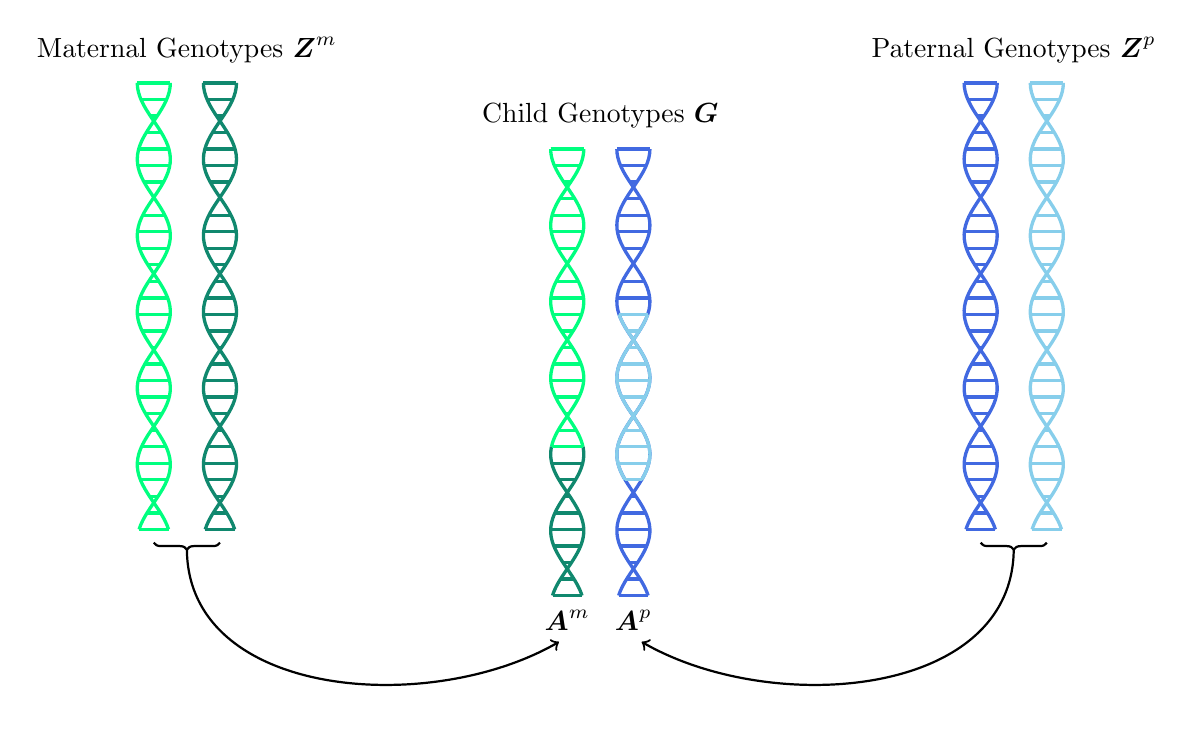
\begin{tikzpicture}[scale=3, rotate=-90]
    \def\zmmx{-3}; % maternal genotype x coordinate
    \def\zmmy{-27}; % maternal genotype y coordinate
    \def\zmpx{-3}; % maternal genotype x coordinate
    \def\zmpy{-23}; % maternal genotype y coordinate
    
    \def\zpmx{-3}; % paternal genotype x coordinate
    \def\zpmy{23}; % paternal genotype y coordinate
    \def\zppx{-3}; % paternal genotype x coordinate
    \def\zppy{27}; % paternal genotype y coordinate
    
    \def\ambx{1}; % child b maternal allele x coordinate
    \def\amby{-2}; % child b maternal allele y coordinate
    \def\apbx{1}; % child b patenral allele x coordinate
    \def\apby{2}; % child b paternal allele y coordinate
    
    \def\mpcol{PineGreen}; % maternal genotypes color
	\def\mmcol{SpringGreen};
	\def\ppcol{SkyBlue}; % paternal genotypes color
	\def\pmcol{RoyalBlue};
    
   
	\begin{scope}[scale=.07, domain=0:27, samples=101]
	
	    % maternal genotypes %%%%%%%%%%%%%%%%%%%%%%%%%%%%%%%%%%%%%%%%%%%%%%%%%%%%%%%%%%%%%%%%%%%%%%%%%
        \draw[\mmcol, very thick] plot (\x + \zmmx, {cos(\x*39) + \zmmy });
        \draw[\mmcol, very thick] plot (\x + \zmmx, {-cos(\x*39) + \zmmy});
        \draw[\mpcol, very thick] plot (\x + \zmpx, {cos(\x*39) + \zmpy });
        \draw[\mpcol, very thick] plot (\x + \zmpx, {-cos(\x*39) + \zmpy});
        % paternal genotypes %%%%%%%%%%%%%%%%%%%%%%%%%%%%%%%%%%%%%%%%%%%%%%%%%%%%%%%%%%%%%%%%%%%%%%%%%
        \draw[\pmcol, very thick] plot (\x + \zpmx, {cos(\x*39) + \zpmy });
        \draw[\pmcol, very thick] plot (\x + \zpmx, {-cos(\x*39) + \zpmy});
        \draw[\ppcol, very thick] plot (\x + \zppx, {cos(\x*39) + \zppy });
        \draw[\ppcol, very thick] plot (\x + \zppx, {-cos(\x*39) + \zppy});
	    
	    % background color %%%%%%%%%%%%%%%%%%%%%%%%%%%%%%%%%%%%%%%%%%%%%%%%%%%%%%%%%%%%%%%%%%%%%%%%%%%
        \foreach \x in {0,1, ...,27}{
          % maternal genotypes 
          \draw[very thick, \mmcol] (\x + \zmmx,{-cos(\x*39) + \zmmy}) -- (\x + \zmmx,{cos(\x*39) + \zmmy});
          \draw[very thick, \mpcol] (\x + \zmpx,{-cos(\x*39) + \zmpy}) -- (\x + \zmpx,{cos(\x*39) + \zmpy});
          % paternal genotypes
          \draw[very thick, \pmcol] (\x + \zpmx,{-cos(\x*39) + \zpmy}) -- (\x + \zpmx,{cos(\x*39) + \zpmy});
          \draw[very thick, \ppcol] (\x + \zppx,{-cos(\x*39) + \zppy}) -- (\x + \zppx,{cos(\x*39) + \zppy});
        }
        % offspring genotypes %%%%%%%%%%%%%%%%%%%%%%%%%%%%%%%%%%%%%%%%%%%%%%%%%%%%%%%%%%%%%%%%%%%%%%%%
        \draw[\mmcol, domain=0:18, very thick] plot (\x + \ambx, {cos(\x*39) + \amby });
        \draw[\mmcol, domain=0:18, very thick] plot (\x + \ambx, {-cos(\x*39) + \amby });
        \draw[\mpcol, domain=18:27, very thick] plot (\x + \ambx, {cos(\x*39) + \amby });
        \draw[\mpcol, domain=18:27, very thick] plot (\x + \ambx, {-cos(\x*39) + \amby });
        \draw[\pmcol, domain=0:27, very thick] plot (\x + \apbx, {cos(\x*39) + \apby });
        \draw[\pmcol, domain=0:27, very thick] plot (\x + \apbx, {-cos(\x*39) + \apby });
        \draw[\ppcol, domain=10:20, very thick] plot (\x + \apbx, {cos(\x*39) + \apby });
        \draw[\ppcol, domain=10:20, very thick] plot (\x + \apbx, {-cos(\x*39) + \apby });
        \foreach \x in {0,1, ...,27}{
          \draw[very thick, \mpcol] (\x + \ambx,{-cos(\x*39) + \amby}) -- (\x + \ambx,{cos(\x*39) + \amby});
          \draw[very thick, \pmcol] (\x + \apbx,{-cos(\x*39) + \apby}) -- (\x + \apbx,{cos(\x*39) + \apby});
        }
        \foreach \x in {0,1, ...,18}{
          \draw[very thick, \mmcol] (\x + \ambx,{-cos(\x*39) + \amby}) -- (\x + \ambx,{cos(\x*39) + \amby});
        }
        \foreach \x in {10,11, ...,20}{
          \draw[very thick, \ppcol] (\x + \apbx,{-cos(\x*39) + \apby}) -- (\x + \apbx,{cos(\x*39) + \apby});
        }       
        % annotations %%%%%%%%%%%%%%%%%%%%%%%%%%%%%%%%%%%%%%%%%%%%%%%%%%%%%%%%%%%%%%%%%%%%%%%%%%%%%%%%%   
        \node at (\zmmx-2, \zmmy/2+\zmpy/2) {Maternal Genotypes $\boldsymbol{Z}^m$};
        \node at (\zpmx-2, \zpmy/2+\zppy/2) {Paternal Genotypes $\boldsymbol{Z}^p$};
        \node at (\ambx-2, \amby/2+\apby/2) {Child Genotypes $\boldsymbol{G}$};
        \node at (\ambx + 28.5, \amby) {$\boldsymbol{A}^m$};
        \node at (\apbx + 28.5, \apby) {$\boldsymbol{A}^p$};
        % braces %%%%%%%%%%%%%%%%%%%%%%%%%%%%%%%%%%%%%%%%%%%%%%%%%%%%%%%%%%%%%%%%%%%%%%%%%%%%%%%%%%%%%%
        \draw[line width = 0.8, decorate, decoration={brace}] (\zmmx+27.8, \zmpy) -- (\zmpx+27.8, \zmmy);
        \draw[line width = 0.8, decorate, decoration={brace}] (\zpmx+27.8, \zppy) -- (\zppx+27.8, \zpmy);
        % arrows %%%%%%%%%%%%%%%%%%%%%%%%%%%%%%%%%%%%%%%%%%%%%%%%%%%%%%%%%%%%%%%%%%%%%%%%%%%%%%%%%%%%%%
        \draw[->, line width = 0.8, color = black] (\zmmx+28.15, \zmmy/2+\zmpy/2) to [out=0,in=-60] (\ambx+29.8, \amby-0.5);
        \draw[->, line width = 0.8, color = black] (\zpmx+28.15, \zpmy/2+\zppy/2) to [out=0,in=60] (\apbx+29.8, \apby+0.5);
        % \draw[->, line width = 0.6, color = black] (\zmmx+26, \zmmy/2+\zmpy/2) to (\ambx-4, \amby);
        % \draw[->, line width = 0.6, color = gray] (\zpmx+26, \zpmy/2+\zppy/2) to (\apbx-4, \apby);
        
    \end{scope}
 	

	
	
\end{tikzpicture}
\end{figure}


\end{document}